\setcounter{page}{1}

\section{Objetivos}
    \begin{itemize}
        \item Diseñar e implementar una red de acuerdo con los requerimientos de un instituto educativo
    \end{itemize}

\section{Introducción}

El diseño de redes es una de las áreas fundamentales dentro del ámbito de las tecnologías de la información, ya que permite conectar de manera eficiente los dispositivos y sistemas de una organización. Este proyecto busca diseñar y simular la infraestructura de red para el instituto “Ing. Fátima Montserrat”, teniendo en cuenta las necesidades específicas de sus principales usuarios: Profesores, Alumnos y Administrativos. Este diseño tiene como objetivo principal garantizar una comunicación fluida, segura y escalable entre los diferentes departamentos.

La dirección IP asignada para el desarrollo de la red es \texttt{192.168.10.0/24}. A partir de este rango, se utilizarán técnicas de subnetting para dividir la red en subredes más pequeñas y manejables. Este proceso es clave para optimizar el uso de direcciones IP, ya que cada subred permitirá segmentar el tráfico y reducir la congestión en la red principal. Adicionalmente, se implementarán VLANs para separar lógicamente el tráfico de cada grupo de usuarios, reforzando la seguridad y mejorando el rendimiento de la red.

El desarrollo del proyecto incluye varios pasos. En primer lugar, se realizará el cálculo de las subredes necesarias para cubrir los requerimientos del instituto, identificando la dirección de red, la dirección de broadcast y el rango de direcciones disponibles para cada subred. Posteriormente, se procederá a la configuración lógica de la red, asignando puertos específicos a cada subred y asegurando que la topología sea sencilla de administrar y mantener. Además, se integrarán servicios básicos como servidores DNS y web, necesarios para el funcionamiento de la red.

Finalmente, se realizará una simulación del diseño propuesto en un entorno virtual, con el fin de verificar su funcionalidad y realizar ajustes antes de su implementación real. Este proceso es crucial para identificar posibles fallos y optimizar el diseño de la red. Al concluir el proyecto, se analizarán los resultados obtenidos y se evaluará la eficiencia del diseño en términos de uso de recursos, seguridad, rendimiento y escalabilidad.


\section{Problemática}
El instituto ``Ing. Fátima Montserrat'' requiere la comunicación, vía red, para miembros de su comunidad de acuerdo con intereses comunes.
Para ello, cuenta con la IP \texttt{192.168.10.0/24} para atender a 3 conjuntos:
    \begin{itemize}
        \item Profesores
        \item Alumnos
        \item Administrativos
    \end{itemize}

Por ahora, cada conjunto contará solo con 2 computadoras y un servidor web distribuidos en 3 pisos: un equipo por piso. A raíz de un análisis previo se propone el empleo de un switch por nivel y estarían enlazados por medio de otro switch ubicado en el nivel 1, como se muestra en la figura \ref{fig:topologia}.

\begin{figure}[H]
    \centering
    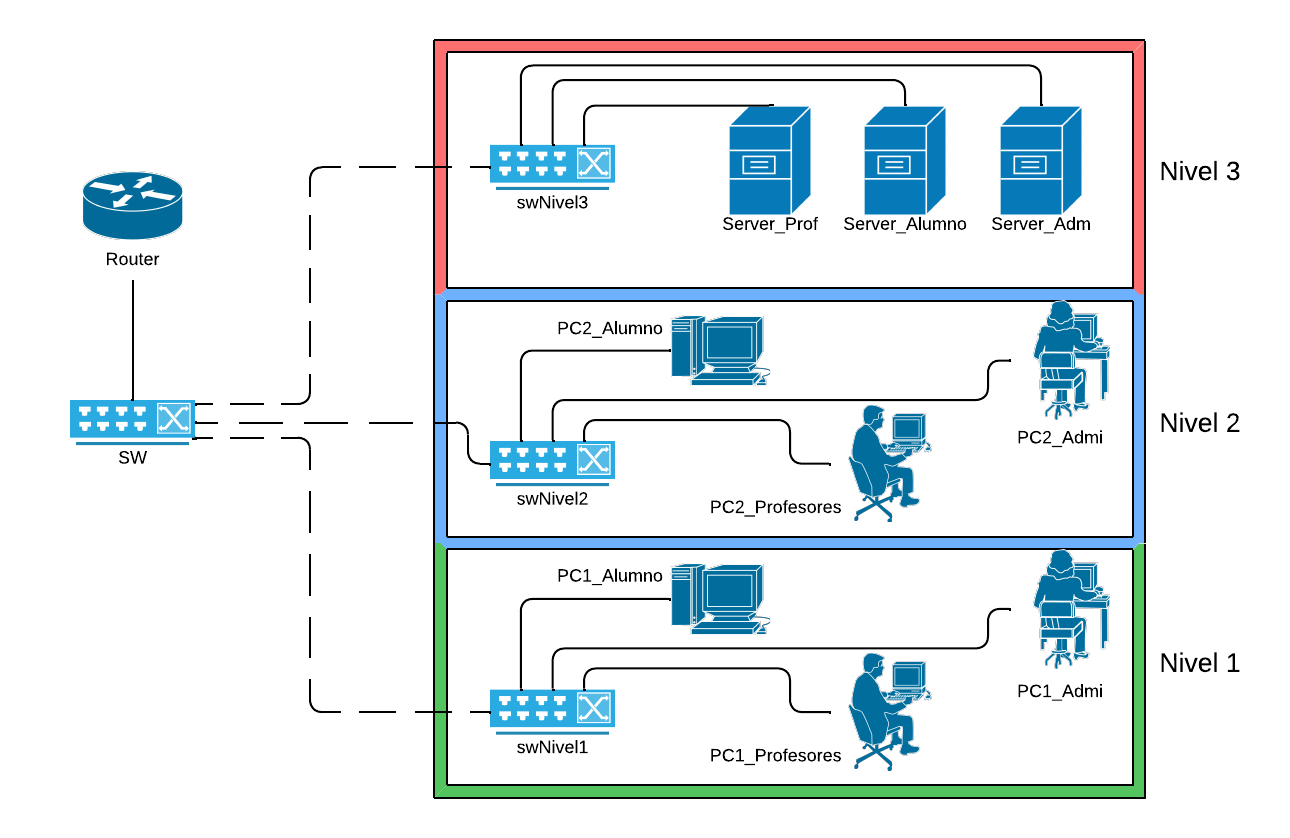
\includegraphics[width=0.6\textwidth]{img/topologia.png}
    \caption{Topología de la red}
    \label{fig:topologia}
\end{figure}

Los switches sugeridos por el consejo técnico del Instituto son cuatro serie 2960 de cisco modelo Ws-c2960 24lc-s y el router Serie 2900.

La asignación de puertos, de acuerdo con los requerimientos, es la siguiente:

\begin{enumerate}
    \item Puerto 1 a 7 para Profesores
    \item Puerto 8 a 15 para Alumnos
    \item Puerto 16 a 23 para Administrativos
\end{enumerate}

Además, durante el diseño se debe contemplar lo siguiente:

\begin{enumerate}
    \item [1] Proponga e implemente el diseño de la solución a este requerimiento en el simulador.
    \item [2] Realice la cotización del material y equipo a emplear. Recuerde que el Instituto ya cuenta con los equipos de cómputo.
    \item [3] Realice los planos de distribución (vista aérea y vista lateral).
\end{enumerate}

\section{Desarrollo del Trabajo}

    \subsection{Cálculo de Subredes}

    Para comenzar con el diseño de la red, se debe obtner las subredes necesarias para la red del instituto. Para ello, se debe calcular la cantidad de bits necesarios para la cantidad de dispositivos que se tienen en cada subred.

    \subsubsection*{Paso 1: Calcular la cantidad de subredes necesarias}

    Para el cálculo de las subredes necesarias, se deben considerar los siguientes aspectos el número total de subredes requeridas. En este caso, utilizaremos 3 subredes (Profesores, Alumnos y Administrativos). Sin embargo, dado que no se suele usar la primera subred en ciertas prácticas, se necesitarán 4 subredes en total

    Para calcular el número de subredes necesarias, utilizamos la siguiente fórmula:

    \begin{equation} 
        2^{n} \geq \text{Número de subredes requeridas} 
    \label{eq:subredes} 
    \end{equation}

    Donde \textbf{n} representa el número de bits que se utilizarán para las subredes adicionales. Al resolver la ecuación, podemos determinar cuántos bits adicionales se necesitan para crear las subredes requeridas.

    \begin{equation} 
        n = log_{2}(\text{Número de subredes requeridas})
    \end{equation}

    Sustituyendo el valor de las subredes requeridas en la ecuación, obtenemos:

    \begin{equation} 
        n = log_{2}(4) = 2
    \end{equation}

    Por lo tanto, se necesitan 2 bits adicionales para crear las subredes requeridas.

    \begin{equation} 
        2^{4} \geq 4 \label{eq:numeroseb} 
    \end{equation}

    \subsubsection*{Paso 2: Obtener la máscara de subred y el rango de direcciones}

    Para calcular el rango de direcciones, primero debemos determinar la máscara de subred. En nuestro ejemplo, la máscara es \texttt{255.255.255.0}, lo que implica que los primeros 16 bits (o tres octetos) están destinados a la parte de la red, y el último octeto está disponible para las direcciones de host.

    Dado que necesitamos 4 subredes, debemos modificar la máscara de red para permitir las subredes. Esto nos lleva a modificar la máscara original agregando 2 bits adicionales. 
    
    \begin{equation*} 
        1111 1111.1111 1111.1111 1111.1100 0000 
    \end{equation*}

    Al convertir el valor binario a decimal, obtenemos la nueva máscara de subred, que es \texttt{255.255.255.192}. Esta máscara de subred permitirá la creación de 4 subredes, cada una con un bloque de 64 direcciones disponibles.
    
    Para calcular el rango entre cada subred, debemos restar el valor del último octeto de la máscara de subred de 256, como se muestra en la ecuación~\ref{eq:rango}.
    
    \begin{equation} 
        \label{eq:rango}
        256 - 192 = 64 
    \end{equation}
    
    Esto significa que cada subred tendrá un bloque de 64 direcciones disponibles. De esta manera, obtenemos el rango de direcciones para cada subred, lo cual es crucial para la asignación de direcciones IP en la red.

    \subsubsection*{Paso 3: Obtener la IP de red y la IP de broadcast}

    Para cada subred, necesitamos determinar la dirección de red y la dirección de broadcast. La dirección de red es la primera dirección de cada subred, mientras que la dirección de broadcast es la última dirección. En la tabla~\ref{tab:VLANs} se las IP's de red y broadcast para cada subred.

    \begin{table}[H]
        \begin{center}
            \begin{tabular}{ c | c | c | c | c }
                \textbf{Subred} & \textbf{Nombre VLAN} & \textbf{IP de Red} & \textbf{Broadcast} & \textbf{Puerto}\\ \hline
                1 & - & 192.168.10.0 & 192.168.10.63 & - \\
                2 & Profesores & 192.168.10.64 & 192.168.10.127 & 1 al 7\\
                3 & Alumnos & 192.168.10.128 & 192.168.10.191 & 8 al 15\\
                4 & Administrativos & 192.168.10.192 & 192.168.10.255 & 16 al 23\\
            \end{tabular}
            \caption{Subredes y VLANs}
            \label{tab:VLANs}
        \end{center}
    \end{table}

    \subsubsection*{Paso 4: Calcular la cantidad de hosts por subred}
    Para calcular el número de hosts disponibles en cada subred, utilizamos la siguiente fórmula:

    \begin{equation}
        \text{Número de hosts por subred} = 2^h - 2
        \label{eq:hosts}
    \end{equation}

    Donde \textbf{h} representa el número de bits disponibles para los hosts en cada subred. Restamos 2 para excluir las direcciones reservadas para la red y el broadcast.
    
    En este caso, la máscara de subred es \textbf{/26}, lo que significa que se han reservado 26 bits para la red, dejando \texttt{32 - 26 = 6} bits para los hosts. Sustituyendo este valor en la ecuación \ref{eq:hosts} obtenemos:
    
    \begin{equation}
        \text{Número de hosts por subred} = 2^6 - 2 = 64 - 2 = 62
    \end{equation}
    
    Por lo tanto, cada subred puede tener un máximo de \textbf{62} hosts disponibles.

    \subsection{Simulación del proyecto}
    \subsubsection*{Asignación de las IPs para cada servicio}

    Para comenzar, se deben asignar las direcciones IP necesarias para cada servicio en la red. En este caso, se necesitan direcciones IP para los servidores web y DNS de cada subred, así como direcciones IP para los servidores DHCP y las puertas de enlace. La tabla~\ref{tab:redes} muestra las direcciones IP asignadas para cada servicio.

    \begin{table}[H]
        \begin{center}
            \begin{tabular}{ c | c | c | c | c }
                \textbf{VLAN} & \textbf{Nombre} & \textbf{IP Servidor web/DNS} & \textbf{IP de red} & \textbf{IP gateway}\\ \hline
                10 & Profesores & 192.168.10.126 & 192.168.10.64 & 192.168.10.65\\
                20 & Alumnos & 192.168.10.190 & 192.168.10.128 & 192.168.10.129\\
                30 & Administrativos & 192.168.10.254 & 192.168.10.192 & 192.168.10.193\\
            \end{tabular}
            \caption{IPs para cada servicio}
            \label{tab:redes}
        \end{center}
    \end{table}


    \subsection*{Diseño del modelo en el simulador}
    Para la simulación de la red, se utilizará el software Cisco Packet Tracer. En la figura~\ref{fig:disSim} se muestra el diseño de la red en el simulador con la topología propuesta.

    \begin{figure}[H]
        \centering
        \includegraphics[width=0.6\textwidth]{img/diseñoSimulador.png}
        \caption{Diseño de la red en el simulador}
        \label{fig:disSim}
    \end{figure}
    
    \subsection*{Asignación de IPs en los servidores Web}

    Para la asignación de IPs en los servidores Web, utilizaremos las direcciones IP que se encuentran en la tabla~\ref{tab:redes}. Además, esta configuración se aplicará a todos los servidores, de manera que la asignación de IPs en los servidores quedaría de la siguiente forma:

    Para el servidor de profesores se asignaró la dirección IP \texttt{192.168.10.126 / 26}, como se muestra en la figura~\ref{fig:serProf_IP}. 
    
    \begin{figure}[H]
        \centering
        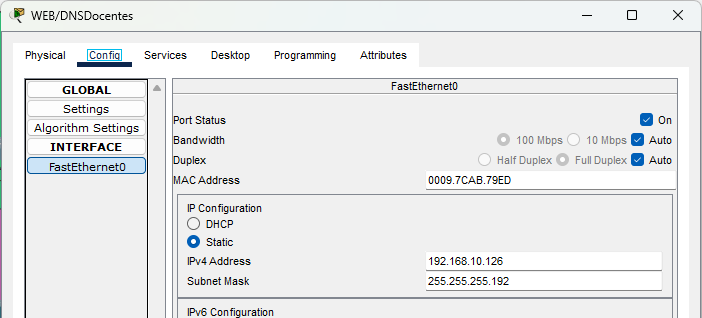
\includegraphics[width=0.7\textwidth]{img/serverprofesores.png}
        \caption{Asignación de IPs en el servidor Web de Profesores}
        \label{fig:serProf_IP}
    \end{figure}

    Para el servidor de estudiantes se asignaró la dirección IP \texttt{192.168.10.190 / 26}, como se muestra en la figura~\ref{fig:serEs_IP}.

    \begin{figure}[H]
        \centering
        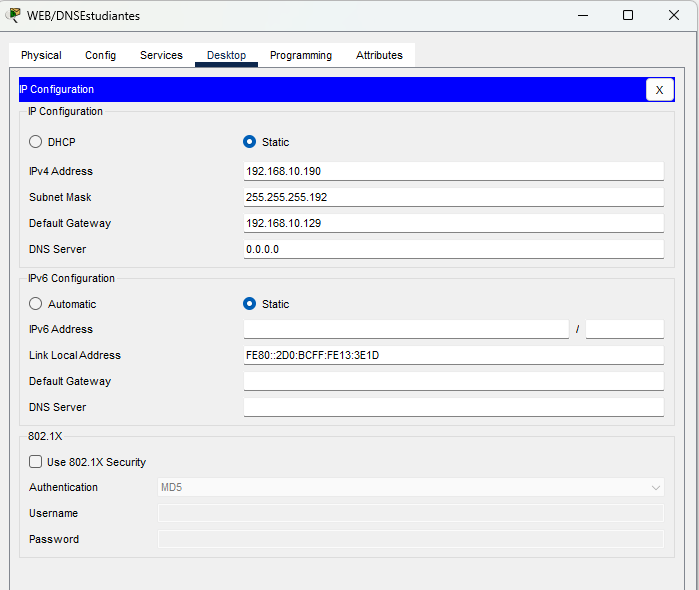
\includegraphics[width=0.7\textwidth]{img/serverestudiantes.png}
        \caption{Asignación de IPs en el servidor Web de Estudiantes}
        \label{fig:serEs_IP}
    \end{figure}

    Para el servidor de administrativos se asignaró la dirección IP \texttt{192.168.10.254 / 26}, como se muestra en la figura~\ref{fig:serAd_IP}.

    \begin{figure}[H]
        \centering
        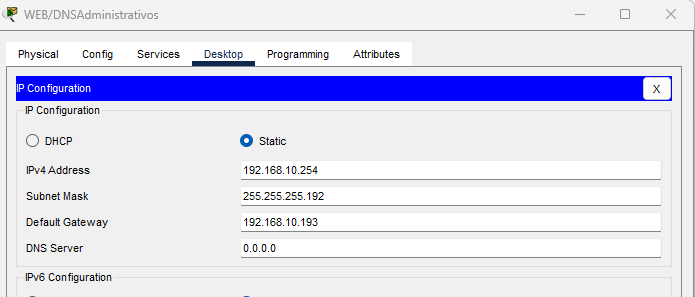
\includegraphics[width=0.7\textwidth]{img/serveradmin.png}
        \caption{Asignación de IPs en el servidor Web de Administrativos}
        \label{fig:serAd_IP}
    \end{figure}

    \subsection*{Asignación del DNS en los servidores Web}
    Para la asignación de DNS, utilizaremos las direcciones IP que se encuentran en el cuadro 2. Además, esta configuración se aplicará a todos los servidores, de manera que la asignación del DNS en los servidores quedaría de la siguiente forma:
    
    \begin{figure}[H]
        \centering
        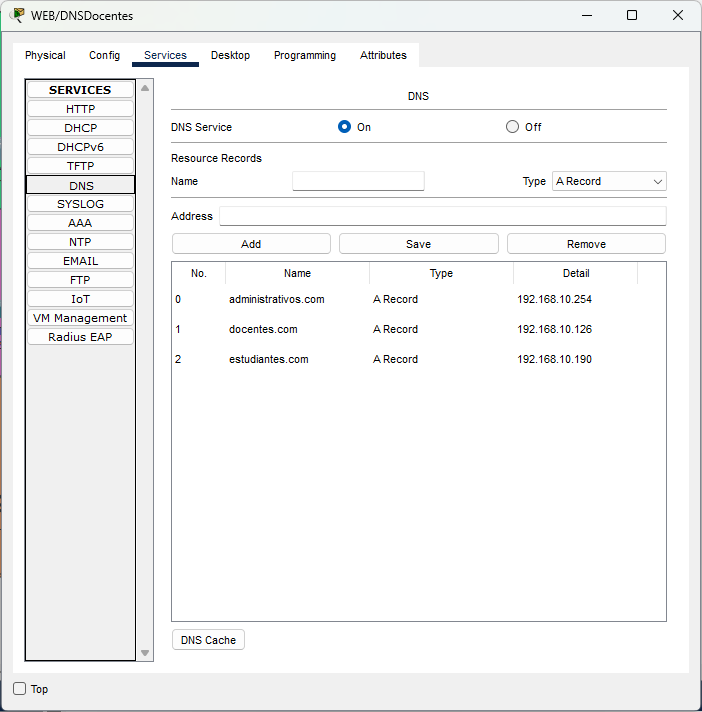
\includegraphics[width=0.7\textwidth]{img/dns.png}
        \caption{Asignación de DNS en todos los servidores Web}
        \label{fig:dns}
    \end{figure}

    \subsection*{Configuración de las VLANs}
    Para la practica utilizaremos los puertos asignados para cada una de las VLANs en cada uno de los switch, de esta forma:
    
    \begin{figure}[H]
        \centering
        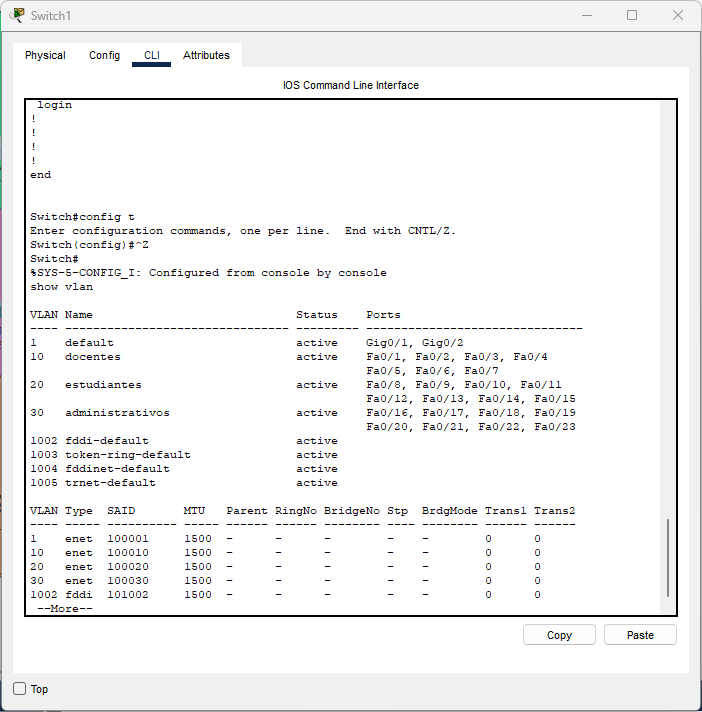
\includegraphics[width=0.6\textwidth]{img/switch1vlan.png}
        \caption{Asignación de puestos en las VLANs Switch 1}
        \label{fig:swvla1}
    \end{figure}
    \begin{figure}[H]
        \centering
        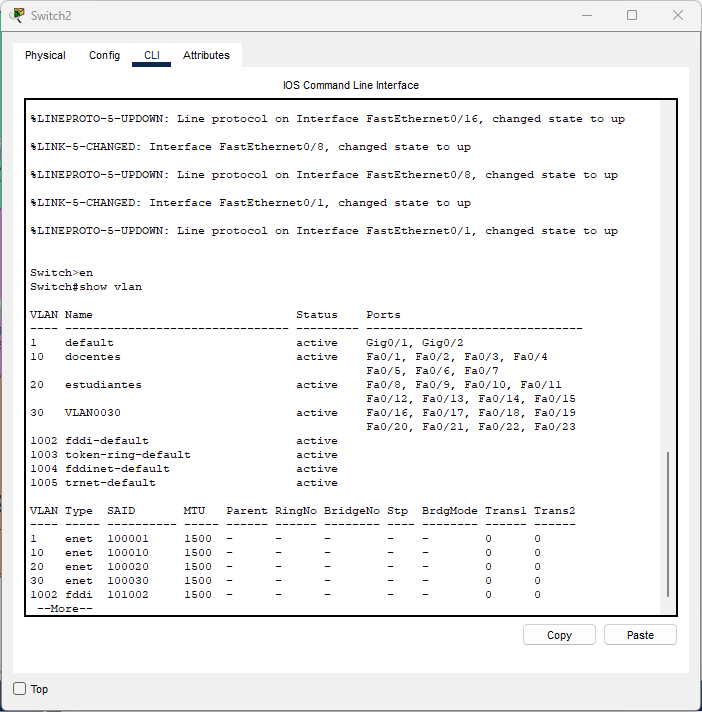
\includegraphics[width=0.6\textwidth]{img/swtichvlan2.png}
        \caption{Asignación de puestos en las VLANs Switch 2}
        \label{fig:swvla2}
    \end{figure}
    \begin{figure}[H]
        \centering
        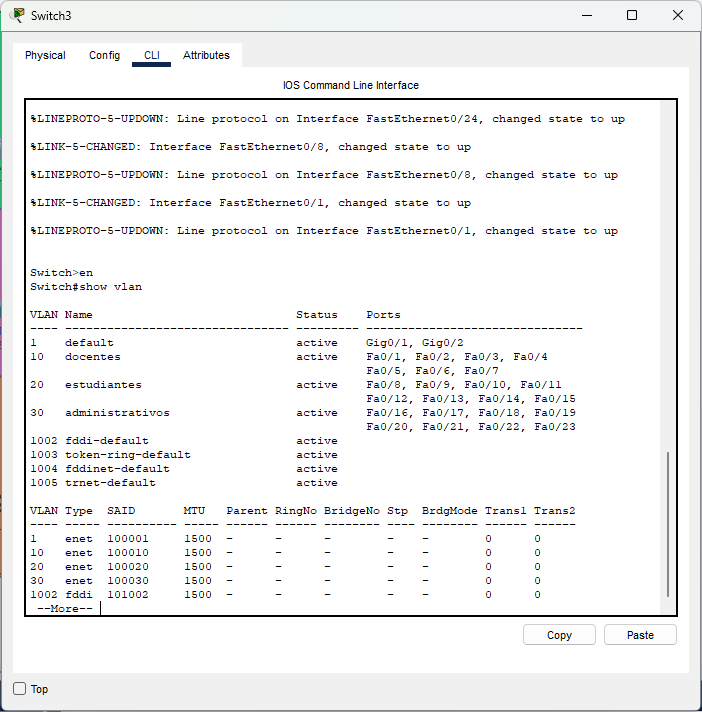
\includegraphics[width=0.6\textwidth]{img/switchvlan3.png}
        \caption{Asignación de puestos en las VLANs Switch 3}
        \label{fig:swvla3}
    \end{figure}
    En el caso del switch 4, no se le asignaron VLANs,  ya que se realizara el troncal de las VLANs y posteriormente conectarse al router.
    \begin{figure}[H]
        \centering
        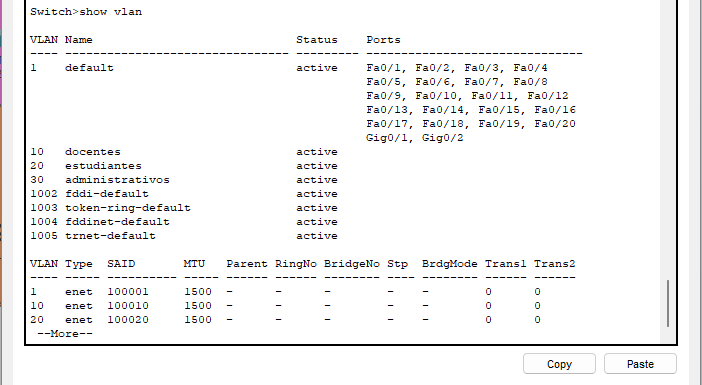
\includegraphics[width=0.6\textwidth]{img/vlansw4.png}
        \caption{Asignación de las VLANs Switch 4}
        \label{fig:swvla4}
    \end{figure}
    \subsection*{Configuración de los trunk en las VLANs}
    La práctica indica la comunicación efectiva entre los switchs por lo que es esencial un buen manejo de los trunk, de forma que los 4 dispositivos deben ser configutados de forma que quede asi:
    
    \begin{figure}[H]
        \centering
        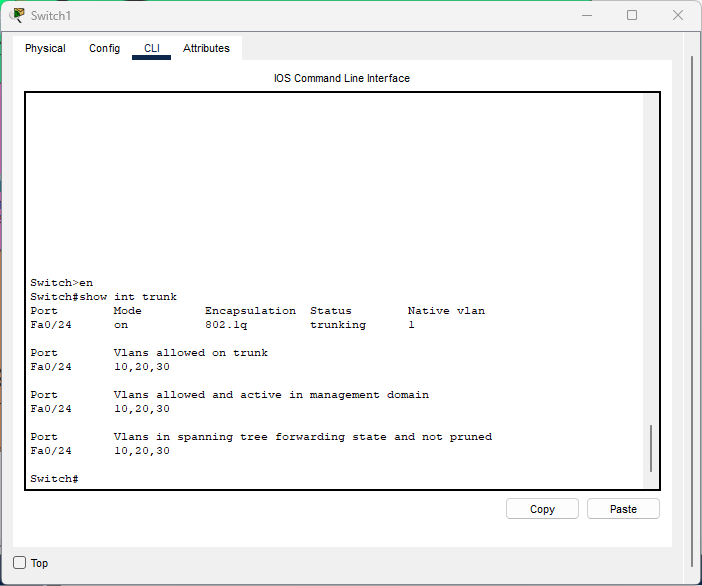
\includegraphics[width=0.6\textwidth]{img/tunksw1.png}
        \caption{Configuración de los trunk en las VLANs Switch 1}
        \label{fig:swtru1}
    \end{figure}
    \begin{figure}[H]
        \centering
        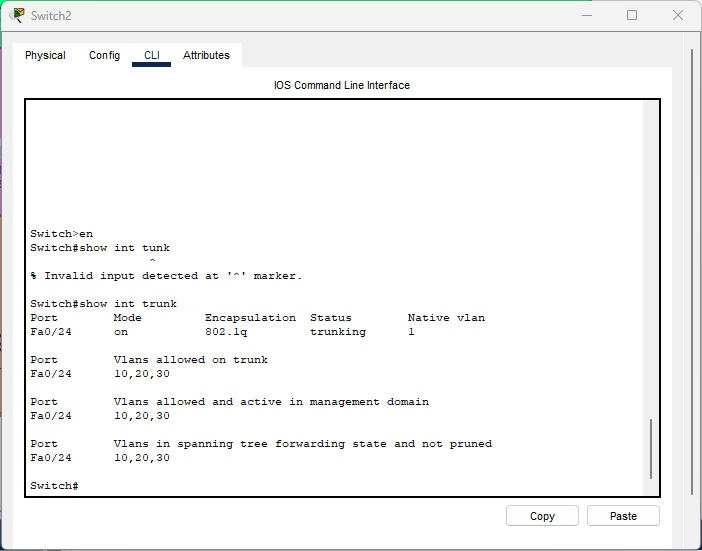
\includegraphics[width=0.6\textwidth]{img/trunksw2.png}
        \caption{Configuración de los trunk en las VLANs Switch 2}
        \label{fig:swtru2}
    \end{figure}
    \begin{figure}[H]
        \centering
        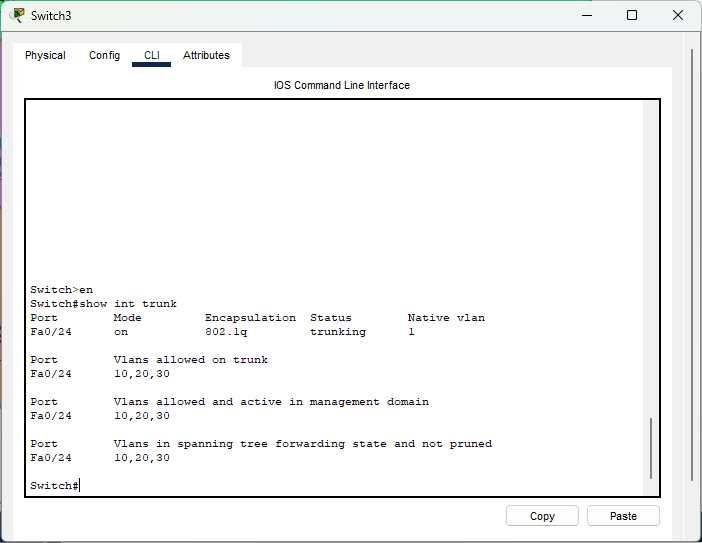
\includegraphics[width=0.6\textwidth]{img/trunk sw3.png}
        \caption{Configuración de los trunk en las VLANs Switch 3}
        \label{fig:swtru3}
    \end{figure}
    \begin{figure}[H]
        \centering
        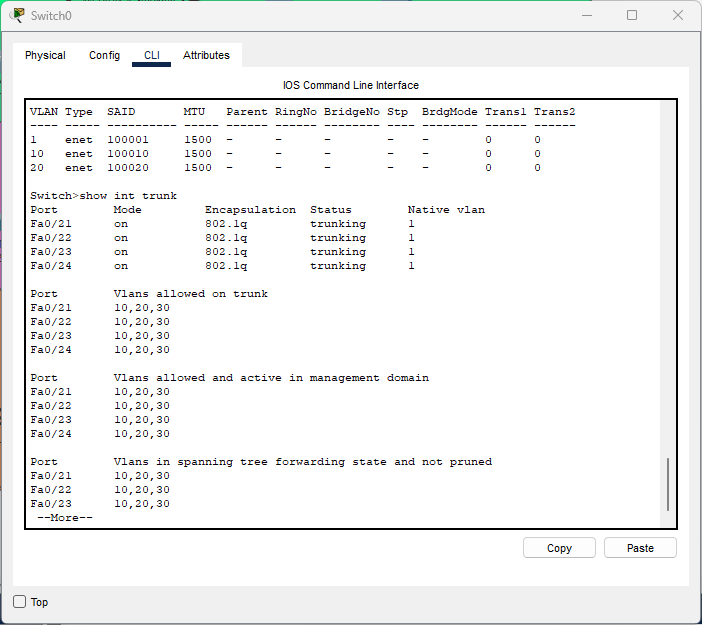
\includegraphics[width=0.6\textwidth]{img/trunsw4.png}
        \caption{Configuración de los trunk en las VLANs Switch 4}
        \label{fig:swtru4}
    \end{figure}
    \subsection*{Configuración del router}
    Para la configuración del router, realizaremos tres acciones principales: primero, asignaremos las puertas de enlace; segundo, excluiremos las direcciones IP necesarias para la red; y tercero, configuraremos el servicio DHCP. De esta forma, el router quedará configurado de la siguiente manera:
    
    \begin{enumerate}
        \item [1] Asignación de las puertas de enlace y de los trunk:
        \begin{figure}[H]
            \centering
            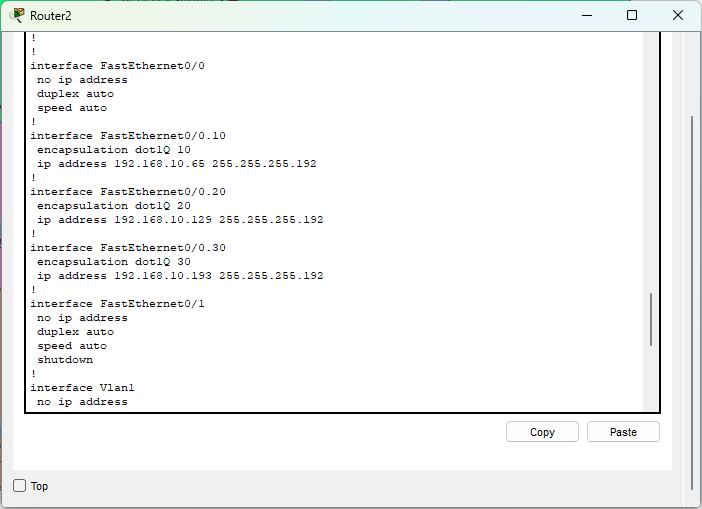
\includegraphics[width=0.6\textwidth]{img/Iprouter.png}
            \caption{Asignación de las puertas de enlace en el router}
            \label{fig:routerip}
        \end{figure}
        
        \item [2] Asignacion del DHCP en el servidor
        
        \begin{figure}[H]
            \centering
            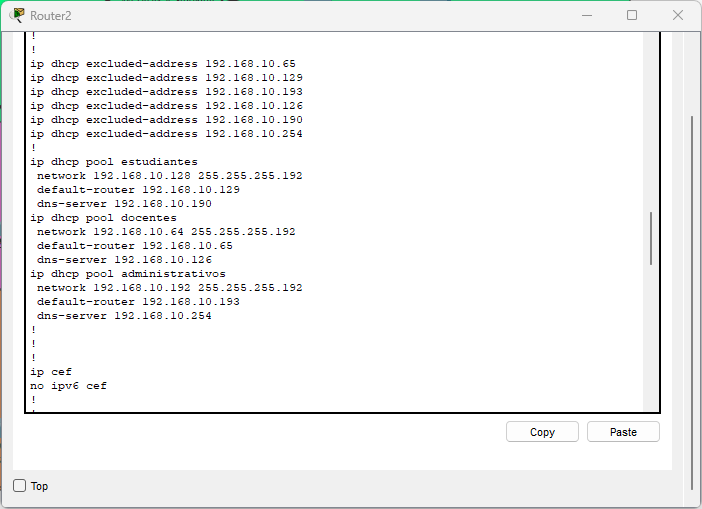
\includegraphics[width=0.6\textwidth]{img/dchpRouter.png}
            \caption{Asignación del DHCP en el router}
            \label{fig:routerDhcp}
        \end{figure}
    
    \end{enumerate}

    En la figura~\ref{fig:routerDhcp} se muestra que se excluyeron las direcciones IP de los servidores web y DNS, así como las puertas de enlace, para evitar que el servidor DHCP asigne estas direcciones a otros dispositivos en la red.

    \subsection*{Prueba del DHCP en los PCs}
    A continuación, se mostrará cómo se asignan las direcciones IP a los PCs de cada subred a través del servicio DHCP.
    \begin{figure}[H]
        \centering
        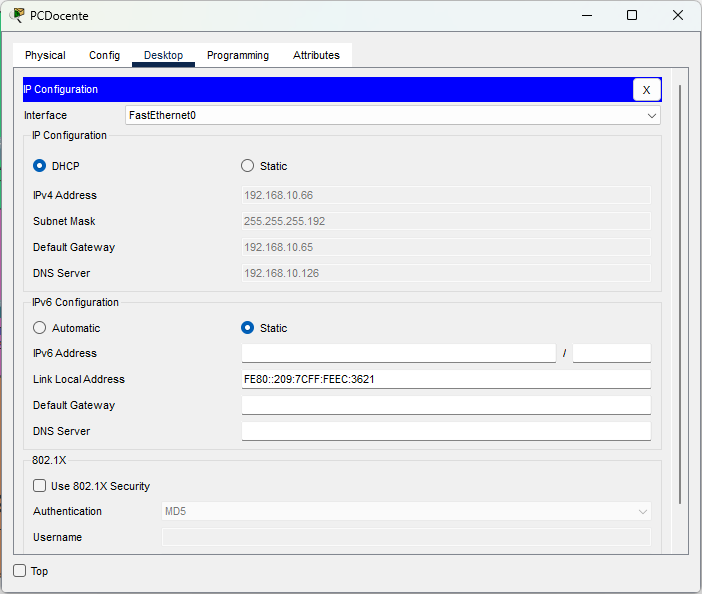
\includegraphics[width=0.6\textwidth]{img/dhcpdoc.png}
        \caption{Asignación del DHCP en el PC del docente}
        \label{fig:pcdDhcp}
    \end{figure}
    \begin{figure}[H]
        \centering
        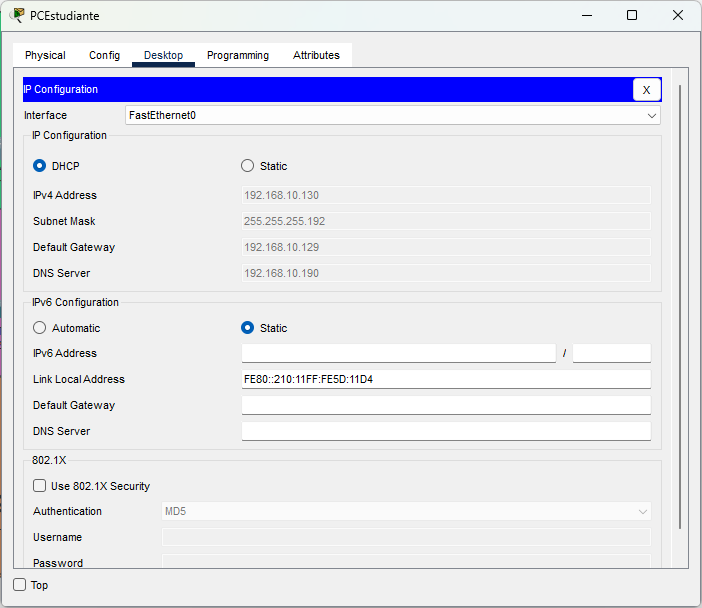
\includegraphics[width=0.6\textwidth]{img/dchpestu.png}
        \caption{Asignación del DHCP en el PC del Estudiante}
        \label{fig:pceDhcp}
    \end{figure}
    \begin{figure}[H]
        \centering
        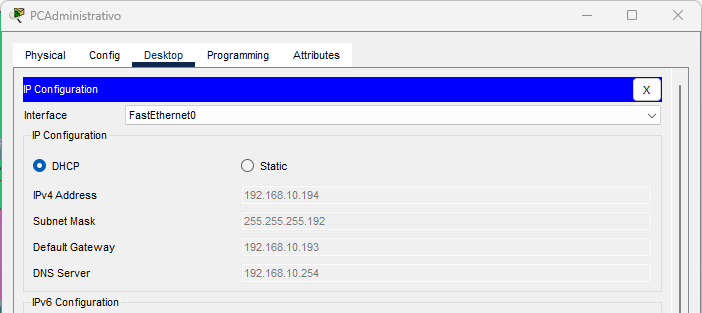
\includegraphics[width=0.6\textwidth]{img/dhcpAdminis.png}
        \caption{Asignación del DHCP en el PC del Administrativo}
        \label{fig:pcADhcp}
    \end{figure}
   
    \subsection*{Prueba del servicio web en los PCs}
    Finalmente, se observa que las páginas web de cada servicio son accesibles desde cualquier PC en las diferentes subredes.
    \begin{figure}[H]
        \centering
        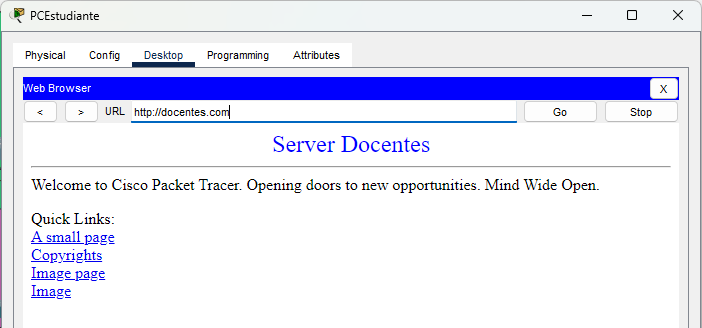
\includegraphics[width=0.6\textwidth]{img/wedDocEs.png}
        \caption{Asignación del servicio web del docente en el PC}
        \label{fig:pcdweb}
    \end{figure}
    \begin{figure}[H]
        \centering
        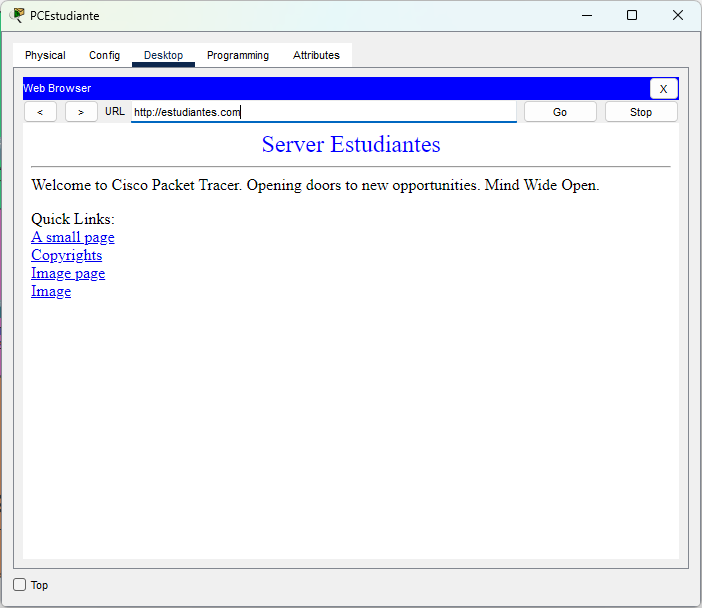
\includegraphics[width=0.6\textwidth]{img/web estudiantes.png}
        \caption{Asignación del servicio web del Estudiante en el PC}
        \label{fig:pceweb}
    \end{figure}
    \begin{figure}[H]
        \centering
        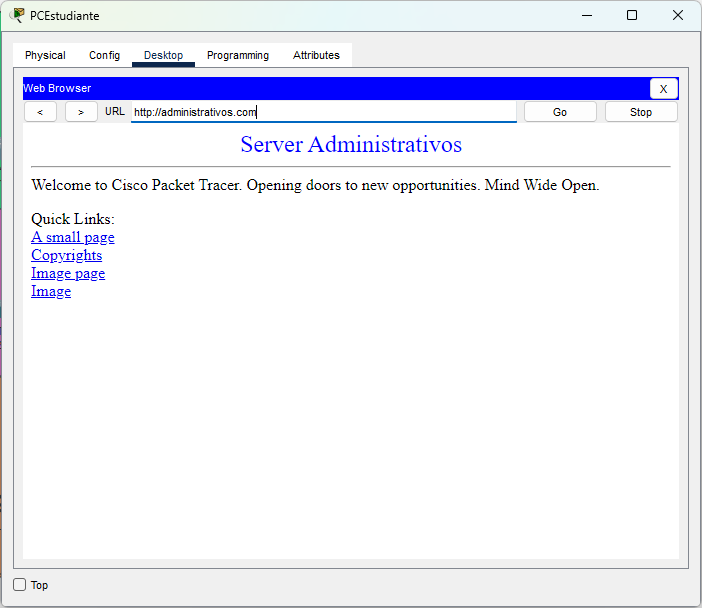
\includegraphics[width=0.6\textwidth]{img/web adminis.png}
        \caption{Asignación del servicio web del Administrativo en el PC}
        \label{fig:pcAweb}
    \end{figure}

    \subsection{Implementación Real de la red}
    \subsubsection*{Configuración de las VLANs en el switch}

    Para comenzar, debemos conectar un extremo de un cable recto al puerto de consola del switch y el otro extremo al puerto serial del PC por medio de un cable RJ45 a DB9. Abrimos el programa HyperTerminal y configuramos el puerto serie con los siguiente parámetros:

    \begin{itemize}
        \item Bits por segundo: 9600
        \item Bits de datos: 8
        \item Paridad: Ninguna
        \item Bits de parada: 1
        \item Control de flujo: Ningu
    \end{itemize}

    \begin{figure}[H]
        \centering
        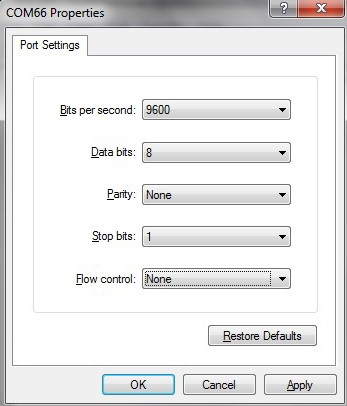
\includegraphics[width=0.6\textwidth]{img/HyperTerminal.jpg}
        \caption{Configuración de HyperTerminal}
        \label{fig:HyperTerminal}
    \end{figure}

    Posteriormente, encendemos el switch y observamos el proceso de arranque. Una vez que el switch ha arrancado, presionamos Enter y ponemos el comando \texttt{enable} para acceder al modo privilegiado. Luego, ingresamos el comando \texttt{configure terminal} para acceder al modo de configuración global.

    A continuación, configuramos las VLANs en el switch. Para ello, utilizamos el comando \texttt{vlan} seguido del número de la VLAN y el nombre de la VLAN. Los comandos para la creación de las VLANs se muestran en el código~\ref{lst:crearVLAN}.

    \begin{lstlisting}[language=bash, caption={Creación de VLANs en el switch}, label={lst:crearVLAN}]
        Switch> enable
        Switch# configure terminal
        Switch(config)# vlan 10
        Switch(config-vlan)# name DOCENTES
        Switch(config-vlan)# vlan 20
        Switch(config-vlan)# name ESTUDIANTES
        Switch(config-vlan)# vlan 30
        Switch(config-vlan)# name ADMINISTRATIVOS
    \end{lstlisting}

    \begin{figure}[H]
        \centering
        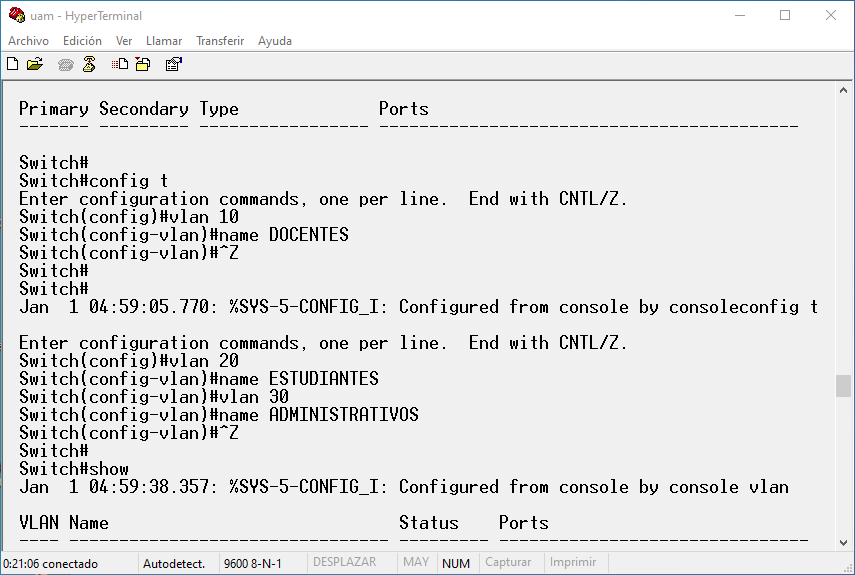
\includegraphics[width=0.6\textwidth]{img/crear_VLAN.png}
        \caption{Creación de VLANs en el switch}
        \label{fig:crearVLAN}
    \end{figure}

    En la figura~\ref{fig:Vlan_creadas} se muestra que las VLANs se han creado correctamente en el switch.

    \begin{figure}[H]
        \centering
        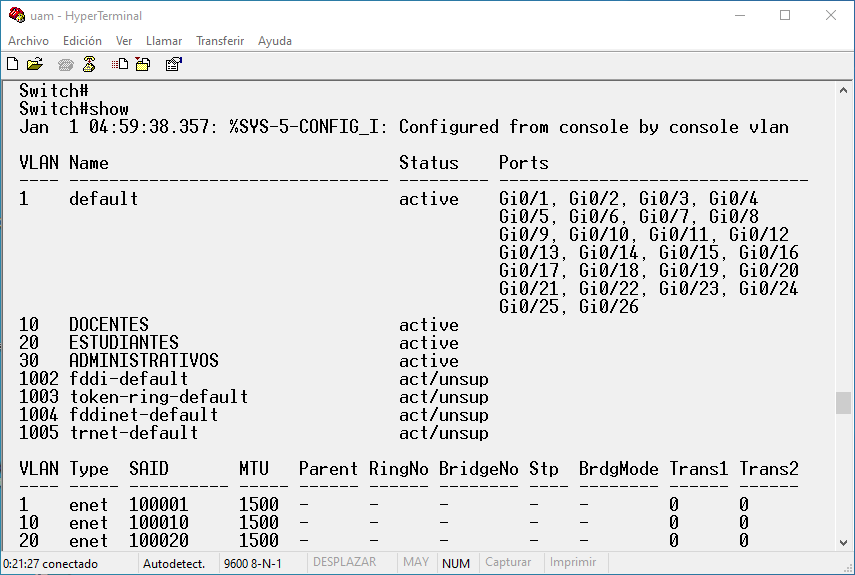
\includegraphics[width=0.6\textwidth]{img/Vlan_creadas.png}
        \caption{VLANs creadas en el switch}
        \label{fig:Vlan_creadas}
    \end{figure}

    A continuación, se procede a asignar los puertos a cada VLAN. Para ello, utilizamos el comando \texttt{interface range} seguido de los puertos que deseamos asignar a la VLAN y el comando \texttt{switchport access vlan} seguido del número de la VLAN. Los comandos para la asignación de puertos a las VLANs se muestran en el código~\ref{lst:asignarVLAN}.

    \begin{lstlisting}[language=bash, caption={Asignación de puertos a las VLANs en el switch}, label={lst:asignarVLAN}]
        Switch> enable
        Switch# configure terminal
        Switch(config)# interface range Gi0/1 - 7
        Switch(config-if-range)# switchport mode access
        Switch(config-if-range)# switchport access vlan 10
        Switch(config)# interface range Gi0/8 - 15
        Switch(config-if-range)# switchport mode access
        Switch(config-if-range)# switchport access vlan 20
        Switch(config)# interface range Gi0/16 - 23
        Switch(config-if-range)# switchport mode access
        Switch(config-if-range)# switchport access vlan 30
    \end{lstlisting}

    \begin{figure}[H]
        \centering
        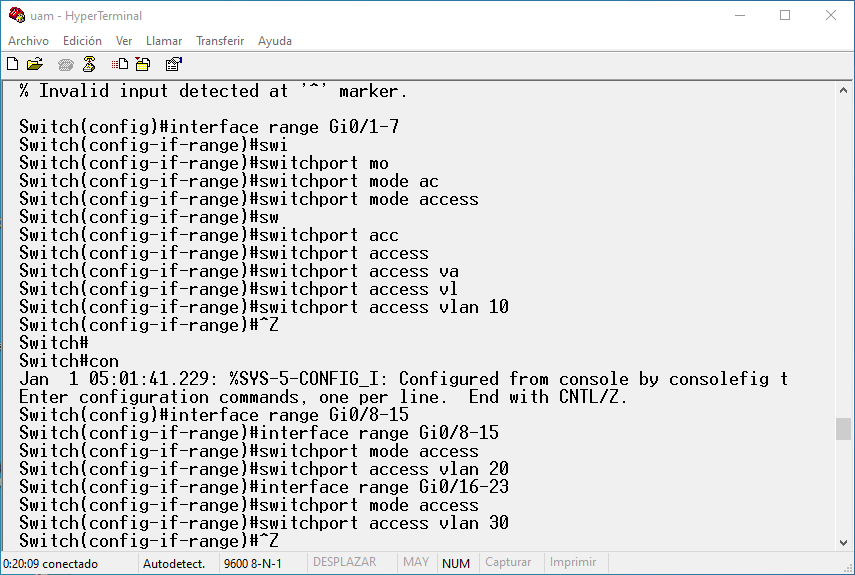
\includegraphics[width=0.6\textwidth]{img/agregar_puertos_VLAN.png}
        \caption{Asignación de puertos a las VLANs en el switch}
        \label{fig:agregar_puertos_VLAN}
    \end{figure}

    Finalmente, verificamos que los puertos hayan  sido asignados correctamente a las VLANs. Para ello, utilizamos el comando \texttt{show vlan brief} para mostrar un resumen de las VLANs y los puertos asignados. En la figura~\ref{fig:puertos_asignados} se muestra que los puertos se han asignado correctamente a las VLANs en el switch.

    \begin{figure}[H]
        \centering
        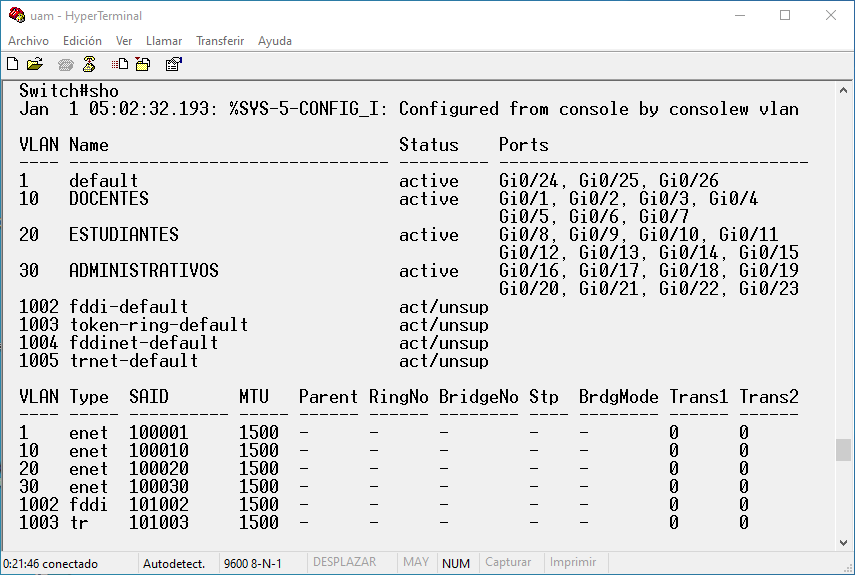
\includegraphics[width=0.6\textwidth]{img/puertos_asignados.png}
        \caption{Puertos asignados a las VLANs en el switch}
        \label{fig:puertos_asignados}
    \end{figure}

    \subsubsection*{Configuración del trunk en el switch}

    Para configurar el trunk en el switch, selecionamos el último puerto del switch y lo configuramos como trunk. Los comandos para la configuración del trunk en el switch se muestran en el código~\ref{lst:configurarTrunk}.

    \begin{lstlisting}[language=bash, caption={Configuración del trunk en el switch}, label={lst:configurarTrunk}]
        Switch> enable
        Switch# configure terminal
        Switch(config)# interface Gi0/24
        Switch(config-if)# switchport mode trunk
        Switch(config-if)# switchport trunk allowed vlan 10,20,30
    \end{lstlisting}

    \subsubsection*{Configuración del router}

    Para configurar el router, primero debemos conectar un extremo de un cable recto al puerto de consola del router y el otro extremo al puerto serial del PC por medio de un cable RJ45 a DB9. Abrimos el programa HyperTerminal y configuramos el puerto serie con los parametros que utilizamos en el switch, como se muestra en la figura~\ref{fig:HyperTerminal}.

    Posteriormente, encendemos el router y observamos el proceso de arranque. Una vez que el router ha arrancado, presionamos Enter y ponemos el comando \texttt{enable} para acceder al modo privilegiado. Luego, ingresamos el comando \texttt{configure terminal} para acceder al modo de configuración global.

    Comenzamos configurando el puerto de la interfaz GigabitEthernet 0/0 del router para que funciene para todas las subredes creadas. Los comandos para la configuración de la interfaz GigabitEthernet 0/0 se muestran en el código~\ref{lst:configurar_router}.

    \begin{lstlisting}[language=bash, caption={Configuración de las interfaces del router}, label={lst:configurar_router}]
        Router> enable
        Router# configure terminal
        Router(config)# interface GigabitEthernet 0/0.10
        Router(config-if)# encapsulation dot1Q 10
        Router(config-if)# ip address 192.168.10.65 255.255.255.192
        Router(config)# interface GigabitEthernet 0/0.20
        Router(config-if)# encapsulation dot1Q 20
        Router(config-if)# ip address 192.168.10.129 255.255.255.192
        Router(config)# interface GigabitEthernet 0/0.30
        Router(config-if)# encapsulation dot1Q 30
        Router(config-if)# ip address 192.168.10.193 255.255.255.192
        Router(config-if)# no shutdown
    \end{lstlisting}

    \begin{figure}[H]
        \centering
        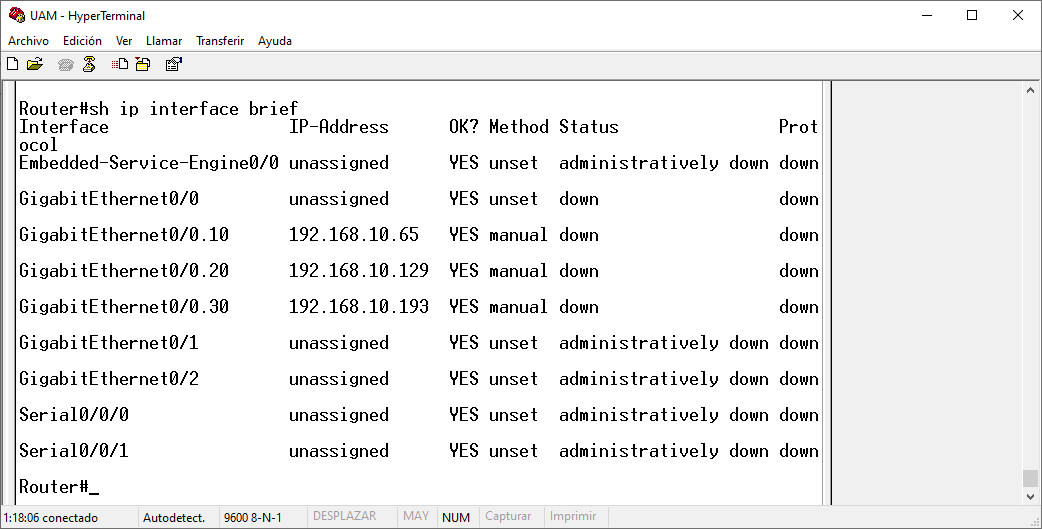
\includegraphics[width=0.6\textwidth]{img/router_VLAN.PNG}
        \caption{Configuración de las interfaces del router}
        \label{fig:configurar_interfaces}
    \end{figure}

    Continuamos con la exclusión de las direcciones IP de los servidores web y DNS, así como las puertas de enlace de cada subred, para evitar que el servidor DHCP asigne estas direcciones a otros dispositivos en la red. Los comandos para la exclusión de direcciones IP se muestran en el código~\ref{lst:excluirIP}.

    \begin{lstlisting}[language=bash, caption={Exclusión de direcciones IP en el router}, label={lst:excluirIP}]
        Router> enable
        Router# configure terminal
        Router(config)# ip dhcp excluded-address 192.168.10.126
        Router(config)# ip dhcp excluded-address 192.168.10.190
        Router(config)# ip dhcp excluded-address 192.168.10.254
        Router(config)# ip dhcp excluded-address 192.168.10.65
        Router(config)# ip dhcp excluded-address 192.168.10.129
        Router(config)# ip dhcp excluded-address 192.168.10.193
    \end{lstlisting}

    Finalmente, configuramos el servicio DHCP en el router para asignar direcciones IP a los dispositivos en la red. Los comandos para la configuración del servicio DHCP se muestran en el código~\ref{lst:configurarDHCP}.

    \begin{lstlisting}[language=bash, caption={Configuración del servicio DHCP en el router}, label={lst:configurarDHCP}]
        Router> enable
        Router# configure terminal
        Router(config)# ip dhcp pool profesores
        Router(dhcp-config)# network 192.168.10.64 255.255.255.192
        Router(dhcp-config)# default-router 192.168.10.65
        Router(dhcp-config)# dns-server 192.168.10.126
        Router(dhcp-config)# exit
        Router(config)# ip dhcp pool estudiantes
        Router(dhcp-config)# network 192.168.10.128 255.255.255.192
        Router(dhcp-config)# default-router 192.168.10.129
        Router(dhcp-config)# dns-server 192.168.10.190
        Router(dhcp-config)# exit
        Router(config)# ip dhcp pool administradores
        Router(dhcp-config)# network 192.168.10.192
        Router(dhcp-config)# default-router network 192.168.10.193
        Router(dhcp-config)# dns-server network 192.168.10.254
        Router(dhcp-config)# exit
    \end{lstlisting}

    En la figura~\ref{fig:configurar_router} se muestra que se excluyeron las direcciones IP de los servidores web/DNS, y las puertas de enlace de las subredes, para evitar que el servidor DHCP asigne estas direcciones a otros dispositivos en la red, así mismo se configuró el servicio DHCP en el router.
    \begin{figure}[H]
        \centering
        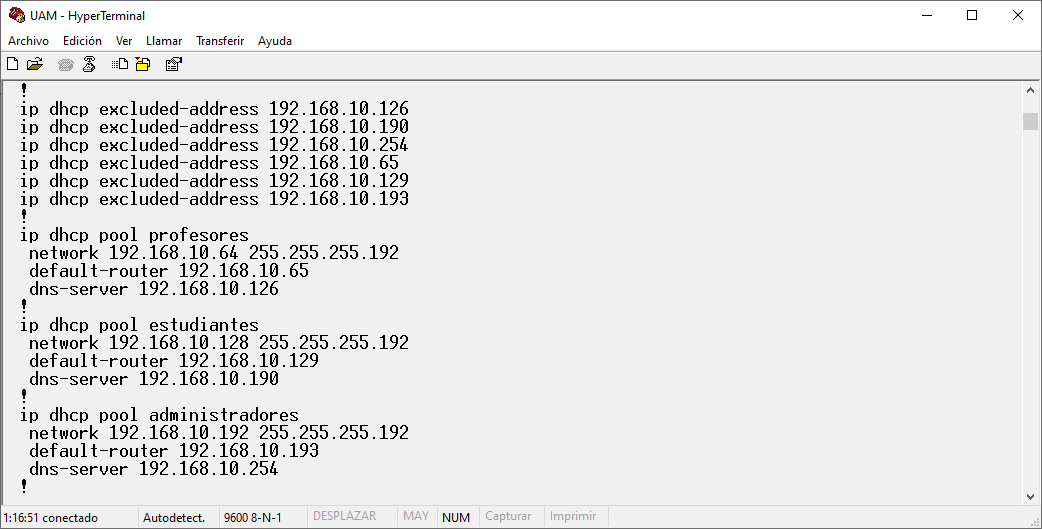
\includegraphics[width=0.6\textwidth]{img/router.PNG}
        \caption{Configuración de las interfaces del router}
        \label{fig:configurar_router}
    \end{figure}

    \subsubsection*{Probar funcionamiento de la red}

    Para probar el funcionamiento de la red, se conectan las computadoras a los puertos asignados en los switches y se verifican las conexiones a los servicios web. En la figura~\ref{fig:funcionamiento_administrativos} se muestra la prueba de conexión al servidor web de Administrativos.

    \begin{figure}[H]
        \centering
        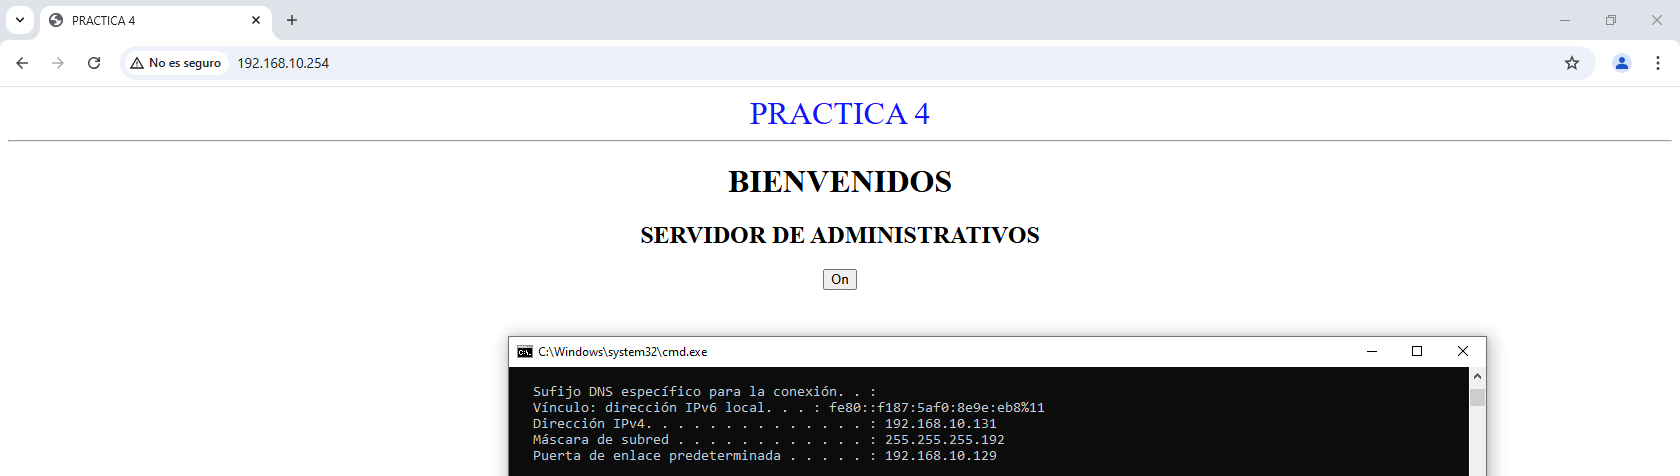
\includegraphics[width=0.6\textwidth]{img/servidor_administrativos.PNG}
        \caption{Prueba de conexión al servidor web de Administrativos}
        \label{fig:funcionamiento_administrativos}
    \end{figure}

    En la figura~\ref{fig:funcionamiento_profesores} se muestra la prueba de conexión al servidor web de Profesores.

    \begin{figure}[H]
        \centering
        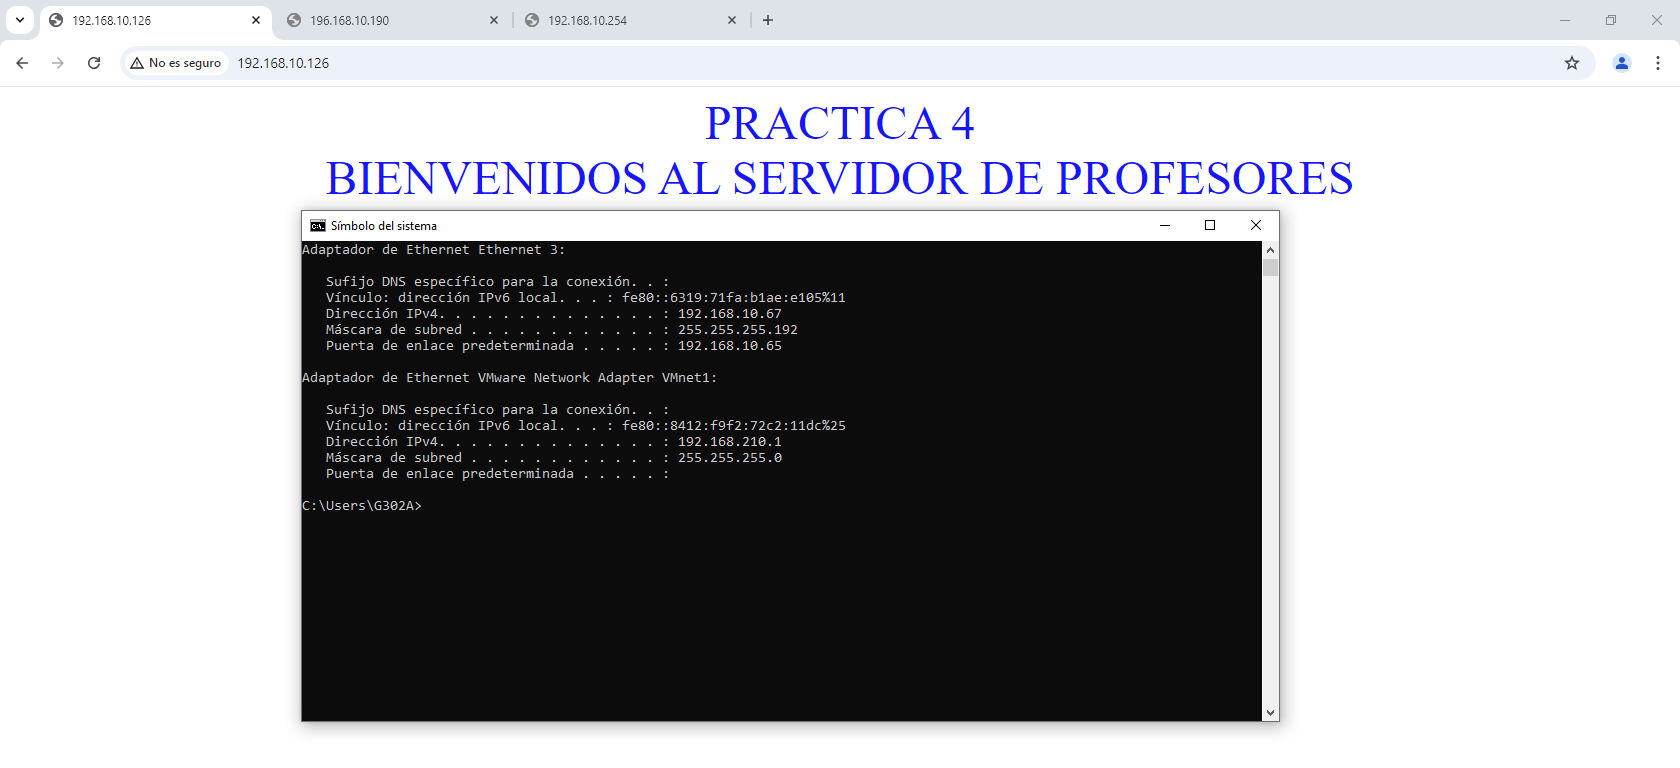
\includegraphics[width=0.6\textwidth]{img/servidor_profesores.PNG}
        \caption{Prueba de conexión al servidor web de Profesores}
        \label{fig:funcionamiento_profesores}
    \end{figure}

    \subsection{Topología de la red}

    Para la creación de los planos de distribución, se conoce que la escuela cuenta con 3 pisos, como se muestra en la figura~\ref{fig:plano_frontal}.

    \begin{figure}[H]
        \centering
        
\includegraphics[width=0.5\textwidth]{img/escuela.png}
        \caption{Vista de frontal de la escuela}
        \label{fig:plano_frontal}
    \end{figure}

    La distribución de los dispositivos en cada piso se ilustra en la figura~\ref{fig:plano_lat}. En los pisos 1 y 2 se ubicará una computadora de cada subred, mientras que en el piso 3 se encontrarán los servidores web y DNS. Cada piso cuenta con un switch, pero el switch principal se encuentra en el piso 1, desde donde conecta con los otros tres switches y el router. Esta distribución se puede ver en la figura~\ref{fig:plano_aereo}.

    \begin{figure}[H]
        \centering
        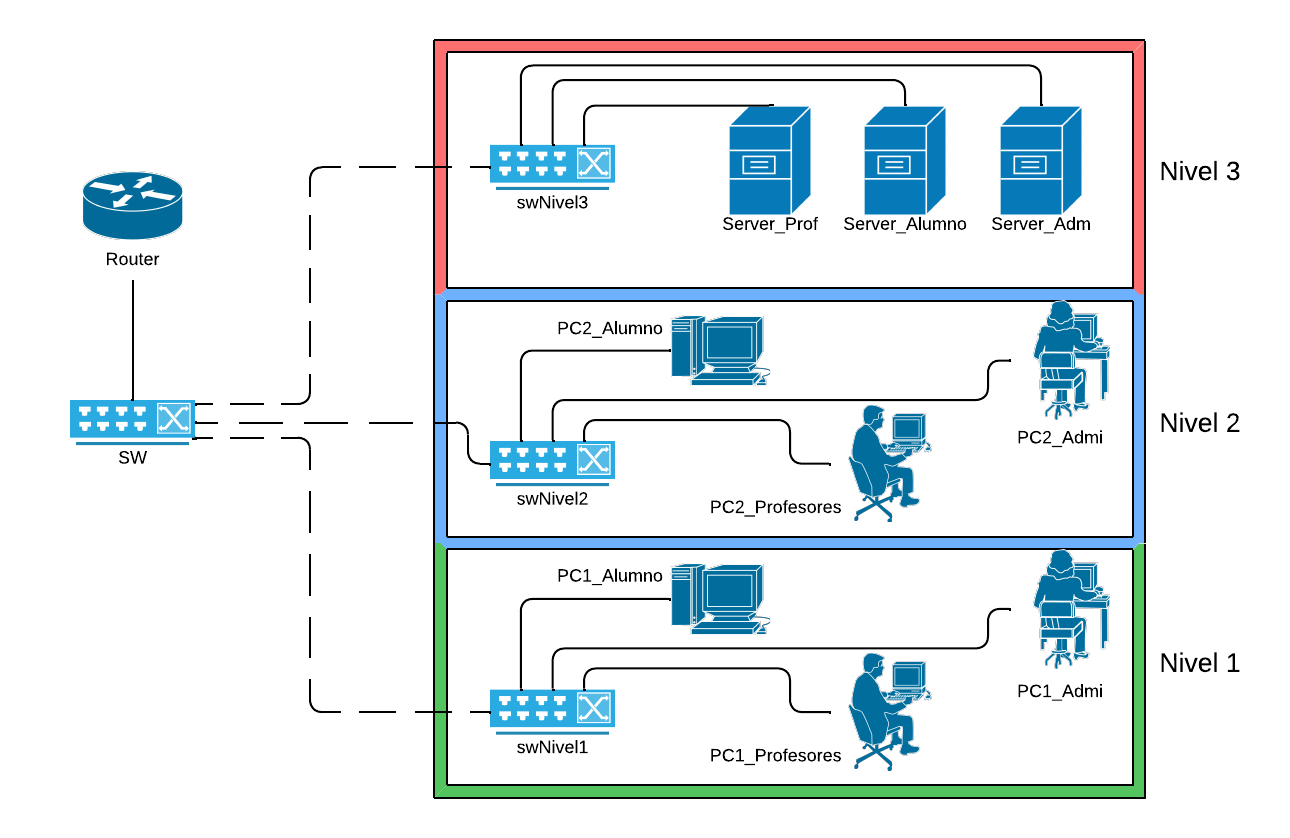
\includegraphics[width=0.8\textwidth]{img/topologia.png}
        \caption{Vista lateral de la distribución de los dispositivos en cada piso}
        \label{fig:plano_lat}
    \end{figure}

    En la figura~\ref{fig:plano_aereo} se muestra la distribución de los dispositivos en cada piso. La linea punteada representa las rejilla que contendrán los cables de red.

    \begin{figure}[H]
        \centering
        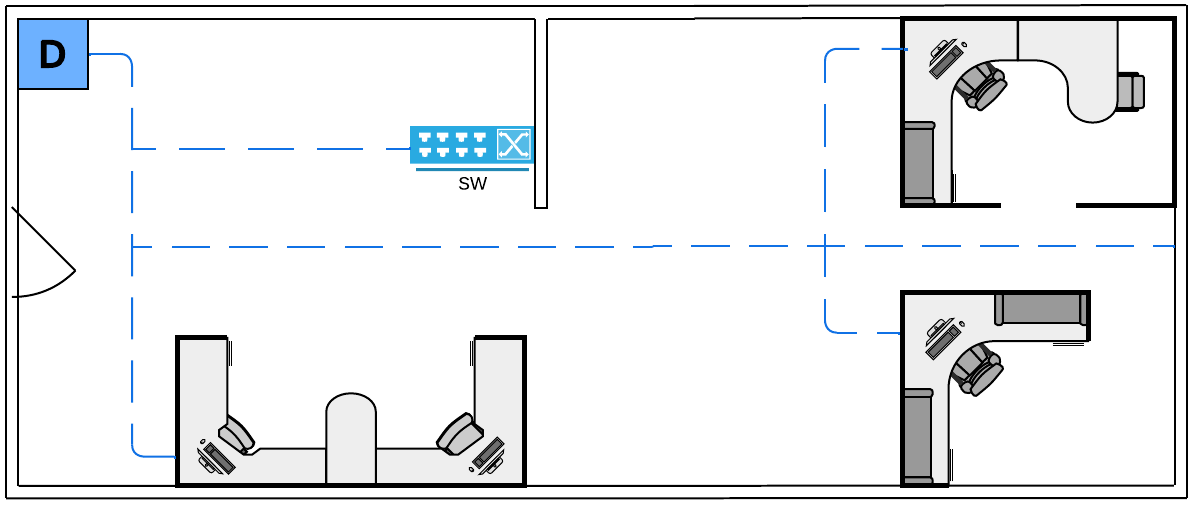
\includegraphics[width=0.8\textwidth]{img/planos.png}
        \caption{Vista aérea de la distribución de los dispositivos en cada piso}
        \label{fig:plano_aereo}
    \end{figure}

    \subsection{Cotización del material y equipo a emplear}

    Se cotizó el material y equipo necesario para la implementación de la red, como se muestra en la tabla~\ref{tab:costos}.
    
    \begin{table}[H]
        \begin{center}
            \begin{tabular}{ c | c | c  }
                \textbf{Cantidad} &\textbf{Producto} & \textbf{Costo}\\ \hline
                2 & Bobinas de cable UTP CAT 6 & 2,537\\
                4 & Switch 2960 & 48,000\\
                1 & Router 2900 & 2900\\
                1 & Pinza ponchadora & 179\\
                1 & Bote de conectores RJ45 & 598\\
                1 & Panel de parcheo, Rack y rejillas & 22,500\\ \hline
            \end{tabular}
            \caption{Cotización del material y equipo a emplear}
            \label{tab:costos}
        \end{center}
    \end{table}
    
    Se utilizará cable UTP CAT 6\cite{cable} de la marca Hikvision debido a que son cables de 100\% cobre, lo que garantiza una mayor calidad y durabilidad. Los switches\cite{switch} y el router\cite{Router} son de la marca Cisco, los conectores RJ45\cite{conectores} son de la marca LinkedPro debido a que tienen chapa de oro.

    Se consideró un estimado de mano de obra de \$500 por hora y se estima que la instalación de la red tomará cerca de 21 horas. Por lo tanto, el costo total de la implementación de la red en el Instituto “Ing. Fátima Montserrat” es de \$87,214.

    Finalmente se realizó la presentación de la cotización y el diseño de la red en clase, como se muestra en la figura~\ref{fig:presentacion}.

    \begin{figure}[H]
        \centering
        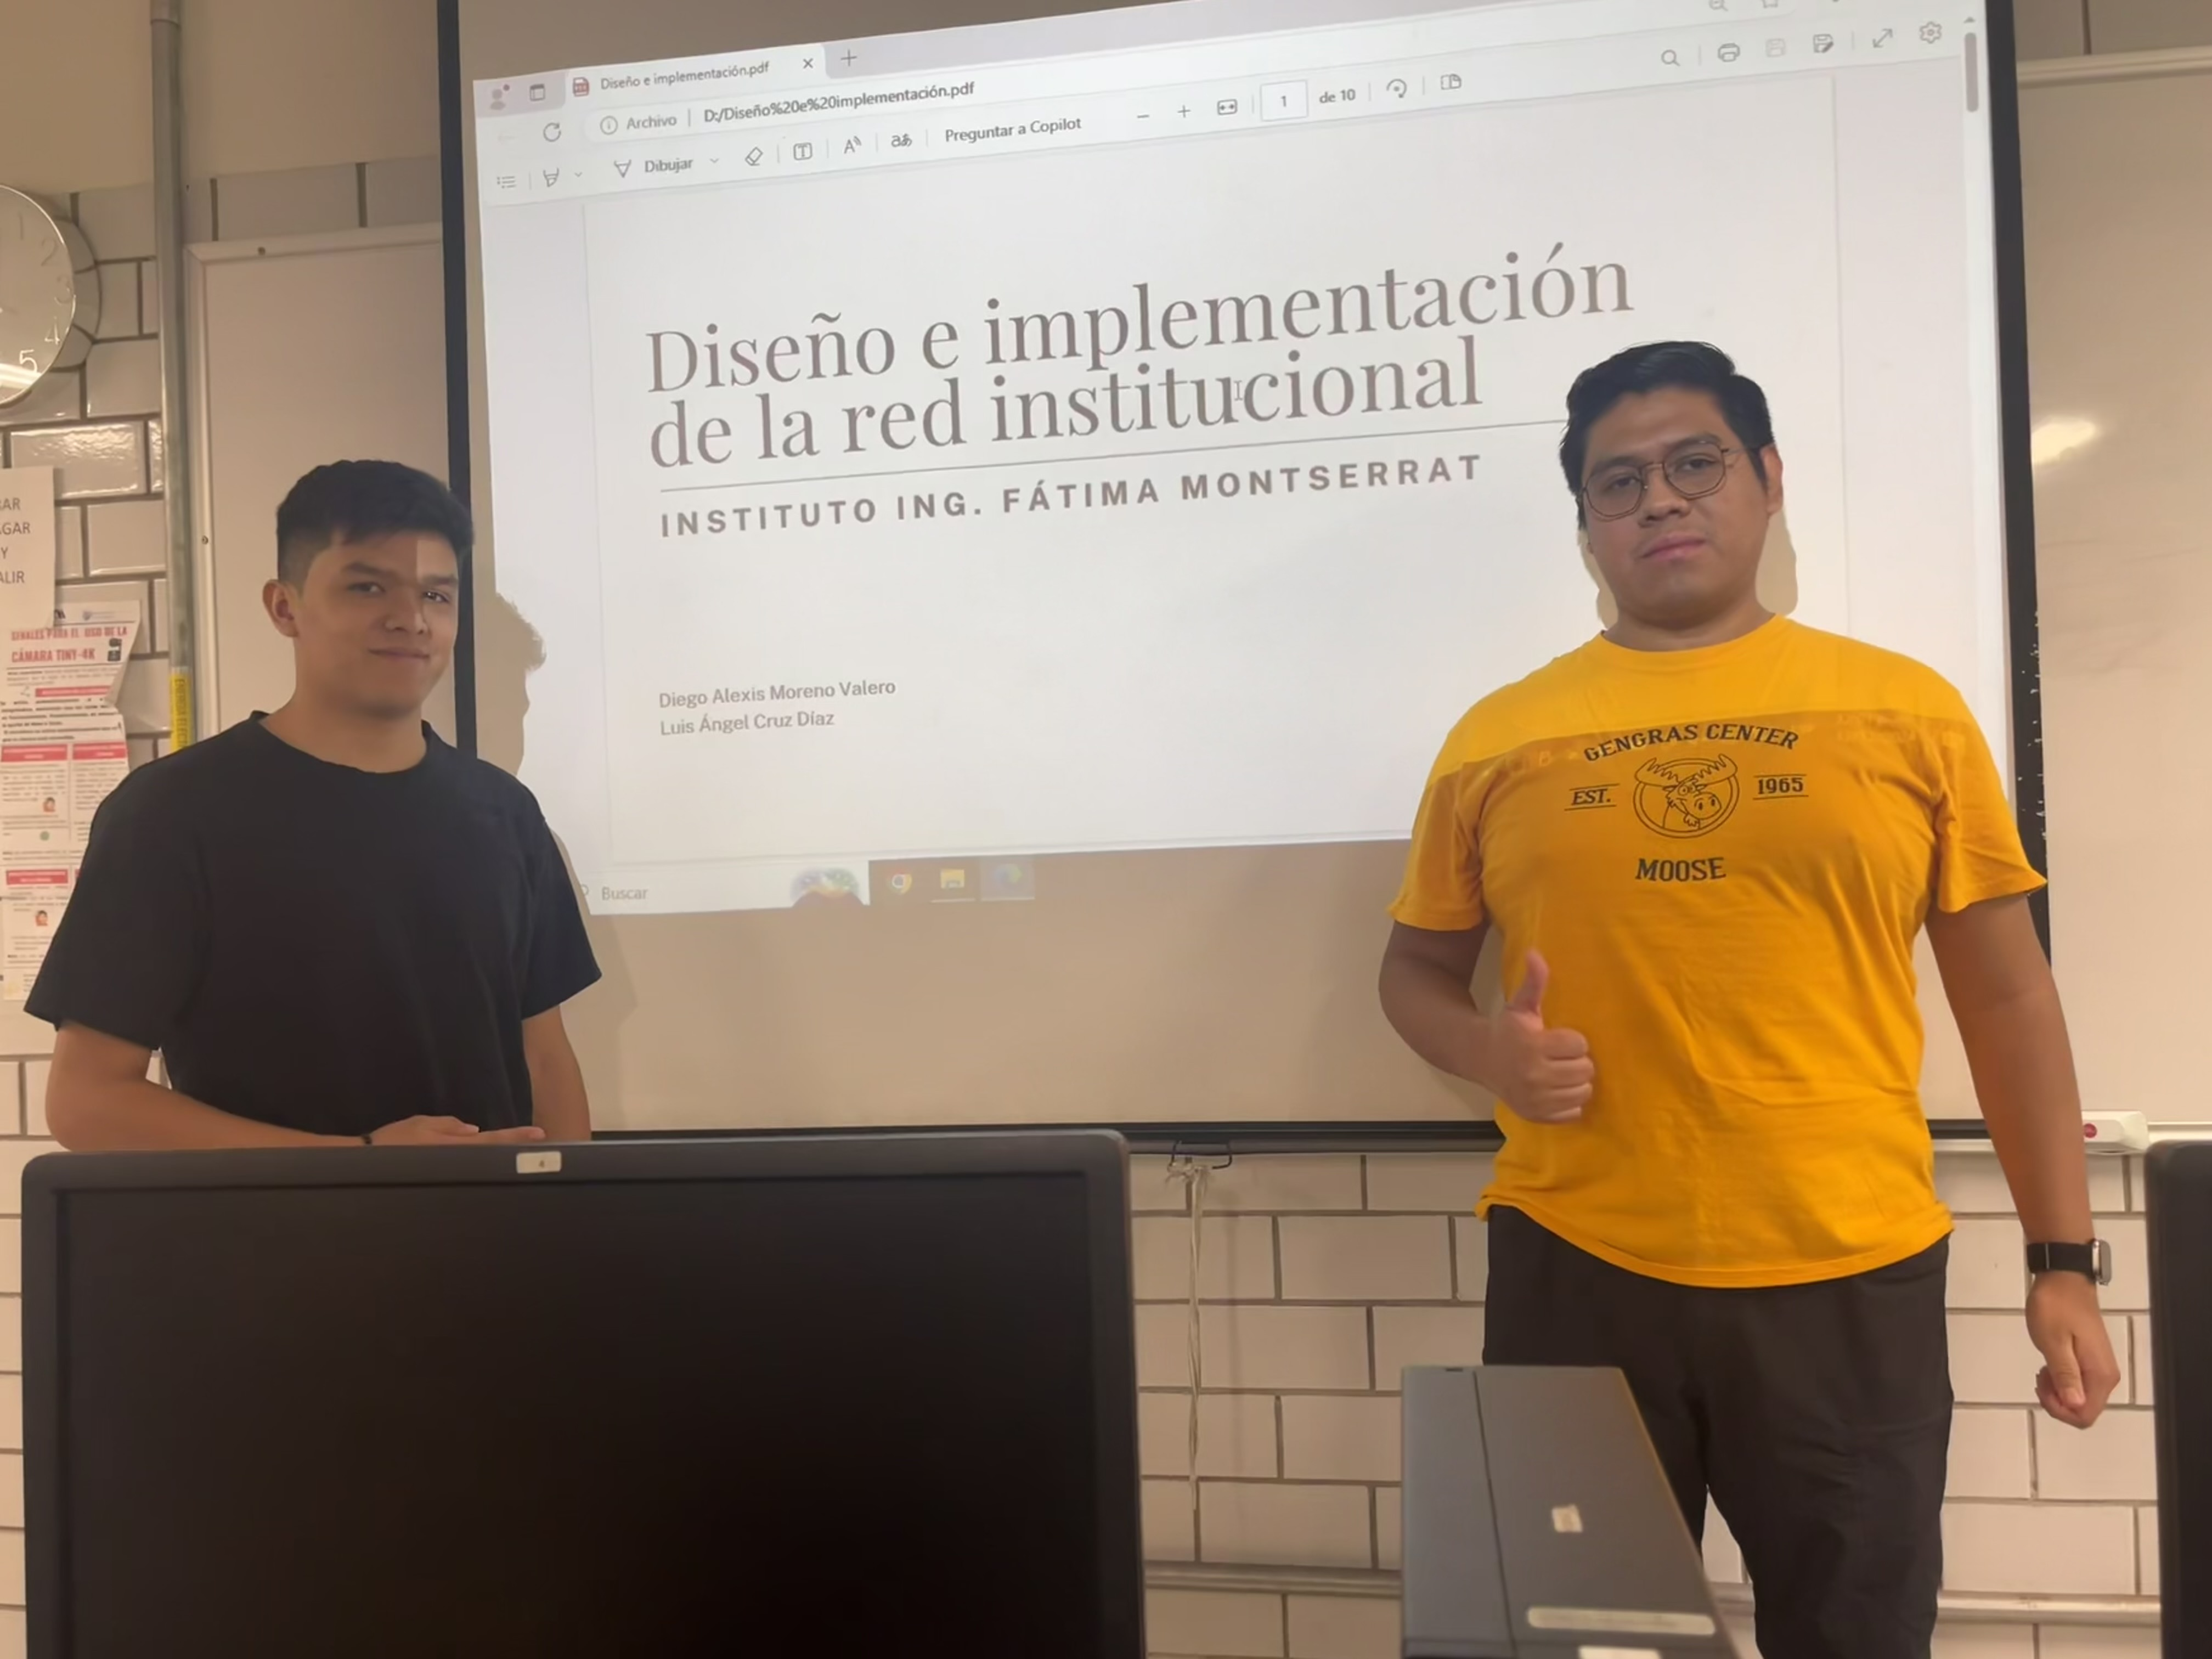
\includegraphics[width=0.6\textwidth]{img/presentacion.jpeg}
        \caption{Presentación de la cotización y el diseño de la red}
        \label{fig:presentacion}
    \end{figure}

\section{Conclusiones}

\begin{itemize}
    \item Luis Ángel Cruz Díaz - 2183038433 \\
    Con la realización de este práctica se logró comprender la importancia de la planificación y diseño de una red institucional, así como la cotización de los materiales y equipo necesarios para su implementación. A través de la simulación y la implementación real de la red, se pudo observar la importancia de la segmentación de la red en VLANs para mejorar la seguridad de la red. Además, se aprendió a configurar el servicios DHCP en un router, así como a asignar direcciones IP de forma dinámica a los dispositivos en la red. Esta práctica permitió aplicar los conocimientos adquiridos durante el curso y reforzar la comprensión de los conceptos de subnetting y VLANs.
    \item Diego Moreno - 2243900185 \\
    El proyecto logró diseñar e implementar una red institucional eficiente y segura, cumpliendo con los requerimientos del Instituto “Ing. Fátima Montserrat”. A través de técnicas de subnetting, VLANs y simulaciones, se optimizó la infraestructura, garantizando escalabilidad y rendimiento. Este ejercicio destacó la importancia de una planificación detallada y pruebas previas para minimizar errores en redes complejas.
\end{itemize}
